\documentclass[../main.tex]{subfiles}
\usepackage{subcaption}

\begin{document}
\section{Experiments -- Task2}

The trained model heavily utilised code provided in ANN-UTADIS.ipynb and helpers.py.
Small changes were introduced to suit the authors' preferences better, but the overall
architecture is based entirely on these snippets.
The model analysed in this section contains 12 hidden layers.

% Perhaps this should be moved if the same technique is used in other places
It is essential to note here that the two cost type criteria: \emph{buying} and \emph{maint}
have been transformed in the following way:
\verb|new_value = 1 - old_value|.
Thanks to this procedure more preferred values are represented by larger numbers,
just as in the case of gain type criteria.
This is done in order to facilitate using non-decreasing marginal value functions for all criteria.

\subsection{Visualizations}
% TODO - add dalex
\begin{figure}[H]
    \centering
    \begin{subfigure}[b]{0.48\linewidth}
        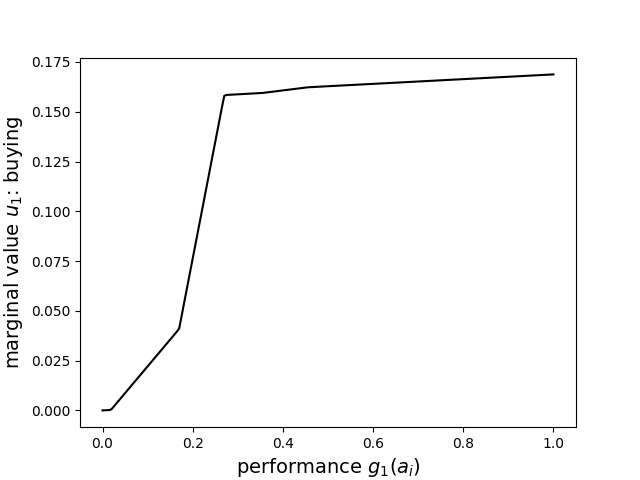
\includegraphics[width=\linewidth]{../img/marginal0.png}
    \end{subfigure}
    \begin{subfigure}[b]{0.48\linewidth}
        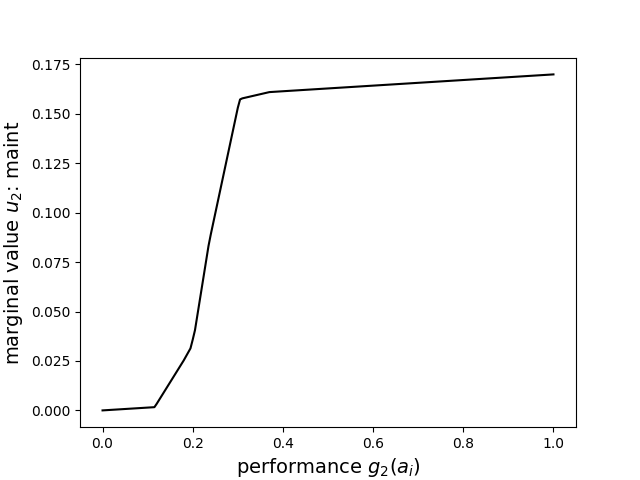
\includegraphics[width=\linewidth]{../img/marginal1.png}
    \end{subfigure}

    \begin{subfigure}[t]{0.48\linewidth}
        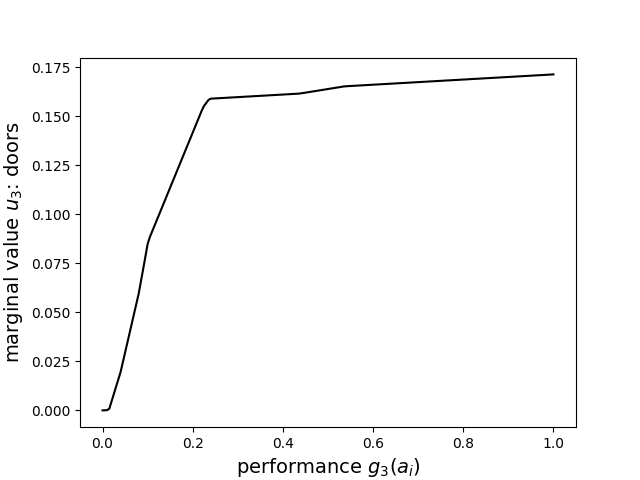
\includegraphics[width=\linewidth]{../img/marginal2.png}

    \end{subfigure}
    \begin{subfigure}[b]{0.48\linewidth}
        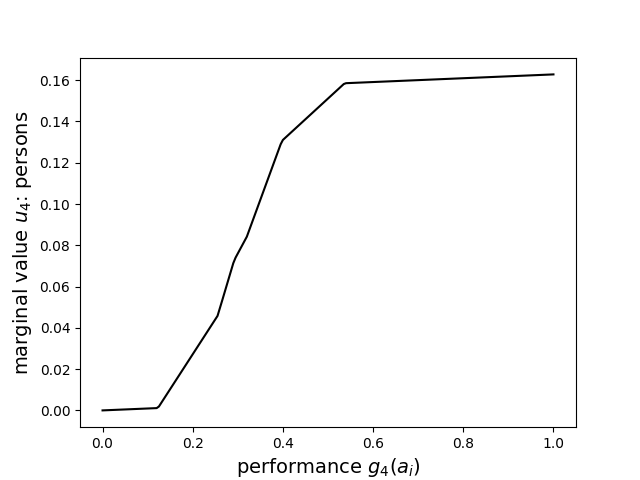
\includegraphics[width=\linewidth]{../img/marginal3.png}
    \end{subfigure}

    \begin{subfigure}[b]{0.48\linewidth}
        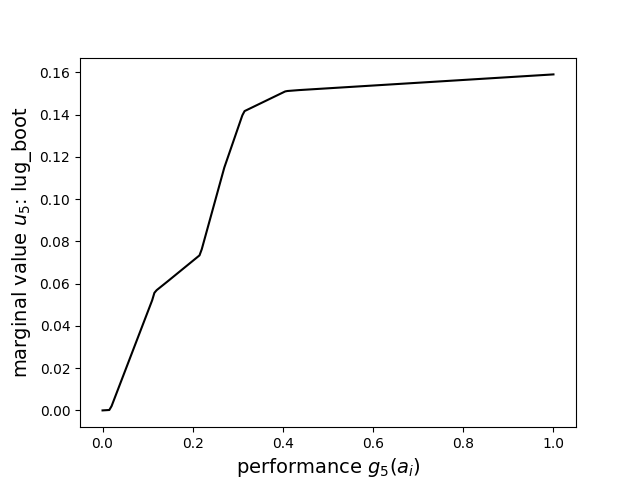
\includegraphics[width=\linewidth]{../img/marginal4.png}
    \end{subfigure}
    \begin{subfigure}[b]{0.48\linewidth}
        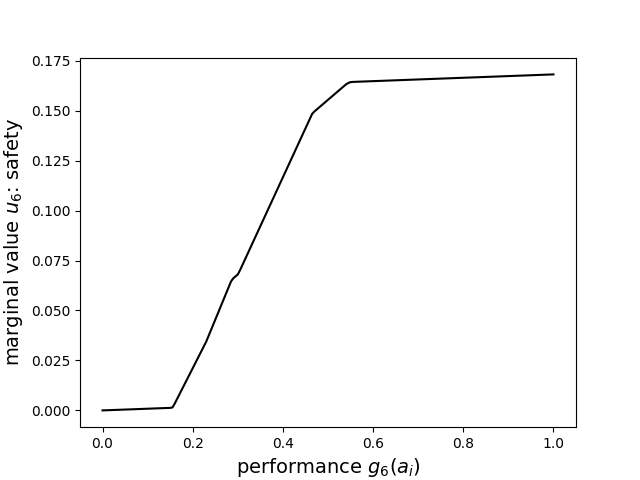
\includegraphics[width=\linewidth]{../img/marginal5.png}
    \end{subfigure}
    \caption{Marginal value functions for all criteria generated by the network}
\end{figure}

\begin{figure}
    \centering
    \begin{subfigure}[b]{\linewidth}
        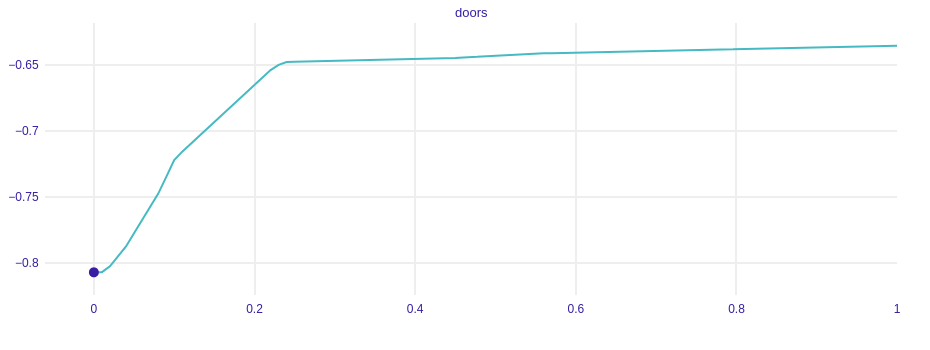
\includegraphics[width=\linewidth]{../img/doors_worst.png}
    \end{subfigure}
    \begin{subfigure}[b]{\linewidth}
        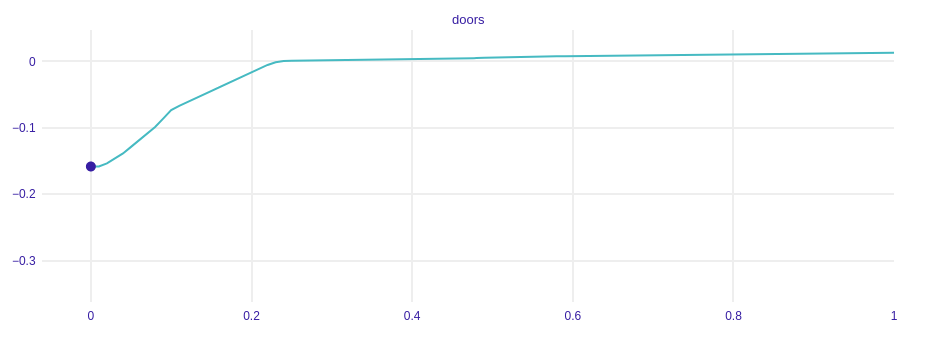
\includegraphics[width=\linewidth]{../img/doors_medium.png}
    \end{subfigure}
    \begin{subfigure}[b]{\linewidth}
        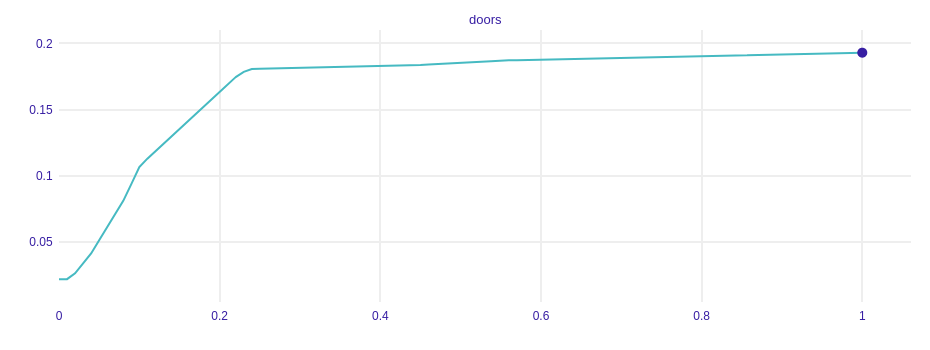
\includegraphics[width=\linewidth]{../img/doors_best.png}
    \end{subfigure}
    \caption{Ceteris paribus analysis for criterion \emph{doors}}
\end{figure}
\subsection{Remarks}


% Based on the parameters obtained, can we say something about the user’s
% preferences? Are there any criteria that have no effect, or have a decisive
% influence? Whether there are any preference thresholds? Are there any
% evaluations on criteria that are indifference in terms of preferences?
No criterion seems to have a decisive influence or be irrelevant.

The maximum values of their marginal value functions ("weights")
are very similar - they are all concentrated roughly between 0.16 and 0.18.

All but one functions are more or less flat for larger values of $g_i$, suggesting
that the decision maker is rather indifferent regarding whether an alternative is
exceptional on one criterion. In other words, the DM is interested in balanced alternatives.
This claim is reinforced by the results of ceteris paribus analysis -
changing the value of just one parameter never has a significant effect on
the model's overall prediction.

% TODO: Add reference to subfigure
% Maybe add discuss more examples?
Having 3 doors seems to be a very big advantage over having only 2,
but adding more doesn't give much benefit

% TODO: discuss minimum change to a criterion that would
% result in assigning na alternative to a different class

% TODO: Interpret the model by at least one...


\end{document}
